\documentclass{article}
\usepackage{mathrsfs}
\usepackage{bm}
\usepackage{amsmath}
\usepackage{amsthm}
\usepackage{amssymb}
\usepackage{graphicx}
\usepackage{float} 
\usepackage{subfigure} 
\usepackage{color}
\usepackage{comment}
%\include{macros}
%\usepackage{floatflt}
%\usepackage{graphics}
%\usepackage{epsfig}


\theoremstyle{definition}
\newtheorem{theorem}{Theorem}[section]
\newtheorem{lemma}[theorem]{Lemma}
\newtheorem{proposition}[theorem]{Proposition}
\newtheorem{corollary}[theorem]{Corollary}

\theoremstyle{definition}
\newtheorem*{defition}{Definition}
\newtheorem*{example}{Example}

\theoremstyle{remark}
\newtheorem*{remark}{Remark}
\newtheorem*{note}{Note}
\newtheorem*{exercise}{Exercise}

\setlength{\oddsidemargin}{-0.25 in}
\setlength{\evensidemargin}{-0.25 in} \setlength{\topmargin}{-0.25
in} \setlength{\textwidth}{7 in} \setlength{\textheight}{8.5 in}
\setlength{\headsep}{0.25 in} \setlength{\parindent}{0 in}
\setlength{\parskip}{0.1 in}

\newcommand{\homework}[5]{
\pagestyle{myheadings} \thispagestyle{plain}
\newpage
\setcounter{page}{1} \setcounter{section}{#5} \noindent
\begin{center}
\framebox{ \vbox{\vspace{2mm} \hbox to 6.28in { {\bf
Part II: Stochastic Programming (Spring 2021) \hfill Homework: 08} }
\vspace{6mm} \hbox to 6.28in { {\Large \hfill #1 \hfill} }
\vspace{6mm} \hbox to 6.28in { {\it Lecturer: #2 \hfill} }
\vspace{2mm} \hbox to 6.28in { {\it \hspace{13mm} #3 \hfill} }
\vspace{2mm} \hbox to 6.28in { {\it Student: #4 \hfill} }
\vspace{2mm} } }
\end{center}
\markboth{#1}{#1} \vspace*{4mm} }


\begin{document}

\homework{Applications of Network Models}
{Junlong Zhang \hspace{5mm} {\tt zhangjunlong@mail.tsinghua.edu.cn}}
{}
{Zhenyu Jin \hspace{11mm} {\tt jzy20@mails.tsinghua.edu.cn}}{8}

\section*{P1.}
\begin{itemize}
	\item Euler's Theorem: A connected graph $G$ possesses an Euler tour 
	(Euler path) if and only if $G$ contains exactly zero (exactly two) 
	nodes of odd degree.
\end{itemize}
\subsection*{Solution:}
\begin{itemize}
	\item If $G$ contains zero node of odd degree, then it can be easily
	proved by mathematical induction.
	\item Under the former condition, when it refers to two node of odd degree,
	then we can add a edge between these two points, and transform $G$ to a graph
	that consists of even degree. Thus if choosing these two points as 
	the origin node and end node, there must exist a path that each edge 
	in $G$ be traveled once. 
\end{itemize}


\section*{P2.}
\begin{itemize}
	\item Notation: Property 1: The optimum traveling salesman 
		  tour does not intersect itself.
\end{itemize}
\subsection*{Solution:}
\begin{itemize}
	\item Suppose that the optimum traveling salesman tour contains two 
		  edges intersect, and the nodes of the two edge are $(a,b)$ and 
		  $(c,d)$. \\
		  In that case, the optimum tour can be improved by changing the 
		  path to $(a,d)$ and $(b, c)$ since the the sum of the diagonal 
		  lengths in the quadrilateral is greater than the sum of the 
		  opposite sides.
\end{itemize}


\section*{Problem 6.1}
\begin{itemize}
	\item (a) If $l(e,f)=-2$, the shortest path from $a$ to $j$ is 
	$a$ \textrightarrow $b$ \textrightarrow $f$ \textrightarrow 
	$e$ \textrightarrow $h$ \textrightarrow $j$, 
	and its value equals to $3+7-2+1+2=11$.
	\item (b) The wrong point of this approach is that this action would 
	make different effects on different number of links of paths. 
	For example, there are two paths A and B, with actual length 5 and 6, 
	and the number of links of them is 2 and 1. Then, we have the processed 
	length of them by this action: A=5+2×2=9 and B=6+2=8. Noted that the 
	action changes the relative length of different paths, hence, the optimal
	solution would not be true.
	
	\item (c) If $l(e,f)=-8$, the shortest path from $a$ to $j$ is $-\infty$, 
	because there exists a negative cycle $f$ \textrightarrow 
	$e$ \textrightarrow $h$ \textrightarrow $f$ with length -1, 
	then we could always pass this cycle to reduce the sum of length of 
	the path. Therefore, the minimum distance between $a$ and $j$ is $-\infty$.
	
	\item (d) If there is a path consists of more than $n-1$ links in the 
	graph with $n$ nodes, then we have that there exists one node which appears 
	at least twice.  However, the goal is minimizing 
	the length of the path. Then we have that the length of this cycle is 
	negative, otherwise, it would not appear in the minimum path. 
	
	\item (e) When there are some negative cycles in a graph, we could find at 
	least one negative number in the diagonal elements of the final 
	matrix $d^(n)$.
	
	\item (f) Initialization:
	\begin{equation}
		\begin{aligned}
			D^0={
			\left[ \begin{array}{ccccc}
				0 & \infty & 3 & \infty & \infty \\
				4 & 0 & \infty & 1 & 2 \\
				3 & 8 & 0 & 2 & 6 \\
				\infty & 1 & \infty & 0 & 4 \\
				\infty & -3 & 6 & 4 & 0
			\end{array} 
			\right ]}, \quad
			P^0={
			\left[ \begin{array}{ccccc}
				- & 1 & 1 & 1 & 1 \\
				2 & - & 2 & 2 & 2 \\
				3 & 3 & - & 3 & 3 \\
				4 & 4 & 4 & - & 4 \\
				5 & 5 & 5 & 5 & -
			\end{array}
			\right ]}
		\end{aligned}
	\end{equation}
	Node 1:
	\begin{equation}
		\begin{aligned}
			D^1={
			\left[ \begin{array}{ccccc}
				0 & \infty & 3 & \infty & \infty \\
				4 & 0 & 7^+ & 1 & 2 \\
				3 & 8 & 0 & 2 & 6 \\
				\infty & 1 & \infty & 0 & 4 \\
				\infty & -3 & 6 & 4 & 0
			\end{array} 
			\right ]}, \quad
			P^1={
			\left[ \begin{array}{ccccc}
				- & 1 & 1 & 1 & 1 \\
				2 & - & 1^+ & 2 & 2 \\
				3 & 3 & - & 3 & 3 \\
				4 & 4 & 4 & - & 4 \\
				5 & 5 & 5 & 5 & -
			\end{array}
			\right ]}
		\end{aligned}
	\end{equation}
	Node 2:
	\begin{equation}
		\begin{aligned}
			D^2={
			\left[ \begin{array}{ccccc}
				0 & \infty & 3 & \infty & \infty \\
				4 & 0 & 7 & 1 & 2 \\
				3 & 8 & 0 & 2 & 6 \\
				5^+ & 1 & 8^+ & 0 & 3^+ \\
				1^+ & -3 & 4^+ & -2^+ & -1^+
			\end{array} 
			\right ]}, \quad
			P^2={
			\left[ \begin{array}{ccccc}
				- & 1 & 1 & 1 & 1 \\
				2 & - & 1 & 2 & 2 \\
				3 & 3 & - & 3 & 3 \\
				2^+ & 4 & 1^+ & - & 2^+ \\
				2^+ & 5 & 1^+ & 2^+ & 2^+
			\end{array}
			\right ]}
		\end{aligned}
	\end{equation}
	Node 3:
	\begin{equation}
		\begin{aligned}
			D^3={
			\left[ \begin{array}{ccccc}
				0 & 11^+ & 3 & 5^+ & 9^+ \\
				4 & 0 & 7 & 1 & 2 \\
				3 & 8 & 0 & 2 & 6 \\
				5 & 1 & 8 & 0 & 3 \\
				1 & -3 & 4 & -2 & -1
			\end{array} 
			\right ]}, \quad
			P^3={
			\left[ \begin{array}{ccccc}
				- & 3^+ & 1 & 3^+ & 3^+ \\
				2 & - & 1 & 2 & 2 \\
				3 & 3 & - & 3 & 3 \\
				2 & 4 & 1 & - & 2 \\
				2 & 5 & 1 & 2 & 2
			\end{array}
			\right ]}
		\end{aligned}
	\end{equation}
	Node 4:
	\begin{equation}
		\begin{aligned}
			D^4={
			\left[ \begin{array}{ccccc}
				0 & 6^+ & 3 & 5 & 8^+ \\
				4 & 0 & 7 & 1 & 2 \\
				3 & 3^+ & 0 & 2 & 5^+ \\
				5 & 1 & 8 & 0 & 3 \\
				1 & -3 & 4 & -2 & -1
			\end{array} 
			\right ]}, \quad
			P^4={
			\left[ \begin{array}{ccccc}
				- & 4^+ & 1 & 3 & 2^+ \\
				2 & - & 1 & 2 & 2 \\
				3 & 4^+ & - & 3 & 2^+ \\
				2 & 4 & 1 & - & 2 \\
				2 & 5 & 1 & 2 & 2
			\end{array}
			\right ]}
		\end{aligned}
	\end{equation}
	Node 5:
	\begin{equation}
		\begin{aligned}
			D^5={
			\left[ \begin{array}{ccccc}
				0 & 5^+ & 3 & 5 & 7^+ \\
				3^+ & -1^+ & 6^+ & 0^+ & 1^+ \\
				3 & 2^+ & 0 & 2 & 4^+ \\
				4^+ & 0^+ & 7^+ & 0 & 2^+ \\
				0^+ & -4^+ & 3^+ & -3^+ & -2^+
			\end{array} 
			\right ]}, \quad
			P^5={
			\left[ \begin{array}{ccccc}
				- & 5^+ & 1 & 3 & 2^+ \\
				2^+ & 5^+ & 1^+ & 2^+ & 2^+ \\
				3 & 5^+ & - & 3 & 2^+ \\
				2^+ & 5^+ & 1^+ & - & 2^+ \\
				2^+ & 5^+ & 1^+ & 2^+ & 2^+
			\end{array}
			\right ]}
		\end{aligned}
	\end{equation}
	\item (g). If there exists some in the graph, we could change the step of
	 making node closed, ensure that nodes could not become closed until all
	  labels are permanent.
	
\end{itemize}


\section*{Problem 6.3}
\begin{itemize}
	\item (a)
	\begin{figure}[H] %H为当前位置,!htb为忽略美学标准,htbp为浮动图形
		\centering %图片居中
		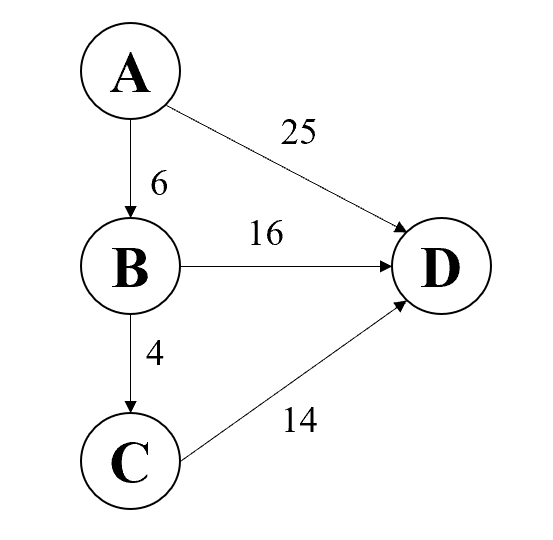
\includegraphics[width=0.5\textwidth]{1.png} %插入图片,[]中设置图片大小,{}中是图片文件名
	\end{figure}
 	\item (b) 
	 \begin{figure}[H] %H为当前位置,!htb为忽略美学标准,htbp为浮动图形
		\centering %图片居中
		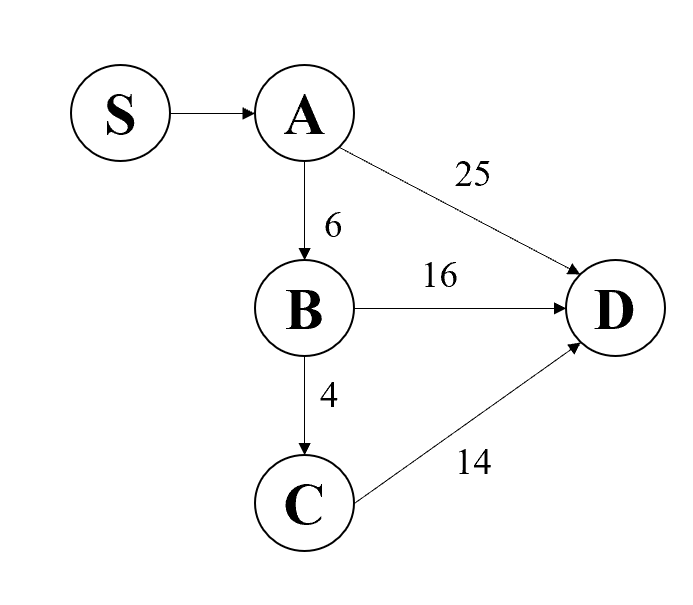
\includegraphics[width=0.5\textwidth]{2.png} %插入图片,[]中设置图片大小,{}中是图片文件名
	\end{figure}
	\item (c) The preferred route in part (a) is choice 2, and the shortest 
	expected travel time is 6+16=22 minutes. The preferred route in part (b) 
	is choice 2, and the shortest expected travel time is 22+5=27 minutes.
	
\end{itemize}


\section*{Problem 6.4}
\begin{itemize}
	\item Noted that the optimal road network should contain a minimum 
	spanning tree to minimize the quantity Z:\\
	\begin{figure}[H] %H为当前位置,!htb为忽略美学标准,htbp为浮动图形
		\centering %图片居中
		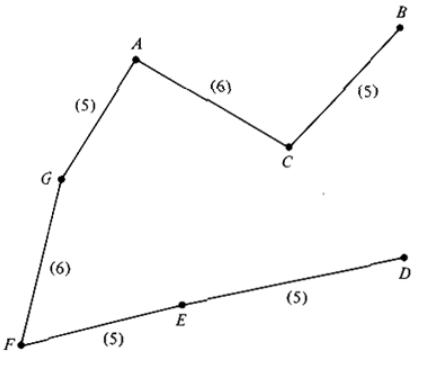
\includegraphics[width=0.5\textwidth]{3.png} %插入图片,[]中设置图片大小,{}中是图片文件名
	\end{figure}
	\item Then the sum of length of this minimize spanning tree is 32 miles, 
	and the upper limit is 34 miles, which means that the minimize 
	spanning tree meets this constrain. Hence, it is the optimal 
	road network.
\end{itemize}


\section*{Problem 6.6}
\begin{itemize}
	\item (a)
		\begin{equation*}
			\begin{aligned}
				\sum_{i \in N} P_i &= \sum_{i \in N} \{(indegree of i) - 
				(outdegree of i)\} \\
				&= \sum_{i \in N}(indegree of i) - \sum_{i \in N}(outdegree of i) \\
				&= \sum_{i \in N} \sum_{(k,i) \in A}1 - \sum_{i \in N} \sum_{(i,k) \in A}1 = 0
			\end{aligned}
		\end{equation*}
	\item (b) 
	In order to have a directed Euler tour, we must have $P_{i}^{'} =0$ for all nodes. Parallel to the $i$
	undirected version, we add artificial arcs $(i, j)$ between supply nodes $i \in S$ and demand nodes
	$j\in D$. Unlike the undirected version, where one additional arc was sufficient to make any
	odd node even, here it may be necessary to add many arcs to a node whose $|P_i|$ is large. In
	order to minimize the total length of arcs added, we construct $\sum_{i \in S}P_i$ minimum distance 
	paths between the supply nodes and demand nodes. In order to ensure $P_{i}^{'}=0$ for all nodes,
	we require $\sum_{j \in D} x_{ij} = P_i$, $\forall i \in S$, which implies that \\
	\begin{center}
		$P_{i}^{'}$= $P_i - $  outdegree of new artificial arcs = $P_i - x_{ij} = 0$ . \\
		$P_{j}^{'} = P_j$ + indegree of new artificial arcs $= P_j + x_{ij} = 0$ .
	\end{center}
	\item (c)
		\begin{itemize}
			\item Step 1: \\
			$S = \{b, d, g\}$ with $P_b = P_d = P_g =1$, and $D = \{a, e\}$ 
			with $P_a = -2, P_e = -1$. By inspection, \\
			\begin{center}
				$d(b, a)=5, d(b, e) = 17
				d(d, a) = 14, d(d, e)=3
				d(g,a) = 20, d(g,e)=9$
			\end{center}
			\item Step 2: \\
			\begin{equation*}
				\begin{aligned}
					minimize   \quad &z = 5x_{ba} + 17x_{be} + 14x_{da}
									+ 3x_{de} + 20x_{ga} + 9x_{ge} \\
				   subject to   \quad &x_{ba} + x_{be} = 1 \\
								&x_{da} + x_{de} = 1 \\
								&x_{ga} + x_{ge} = 1 \\
								&x_{ba} + x_{da} + x_{ga} = 2 \\
								&x_{be} + x_{de} + x_{ge} = 1 \\
								&x_{ij} \in \{0, 1, 2,...\}						
				\end{aligned}
			\end{equation*}
			\item Step3: \\
			$b$ \textrightarrow $a$ \textrightarrow $c$ 
			\textrightarrow $d$ \textrightarrow $c$ \textrightarrow $f$ 
			\textrightarrow $g$ \textrightarrow $d$ \textrightarrow $e$ 
			\textrightarrow $g$ \textrightarrow $d$ \textrightarrow $e$
			\textrightarrow $b$ \textrightarrow $a$ \textrightarrow $d$
			\textrightarrow $e$ \textrightarrow $b$ \textrightarrow $a$ 
			\textrightarrow $b$ is one possible tour.
		\end{itemize}
	\item (d) The suggested method forces us to traverse every undirected arc twice (once in each direction),
	which may not be optimal.
\end{itemize}


















\end{document}